The model is based on research on the ant Lasius niger, in the book "Self-organization in biological systems" \citep{camazine2003}. This paper describes the process of trail formation in ants. This phenomenon can easily be observed in the wild, by placing some sugar solution. After a short while the food will be discovered and shortly after, the number of ants at the food source will increase rapidly, until eventually it stabilizes and a well established trail of ants can be observed from the nest to the sugar. To study this behaviour, several experiments have been conducted on a colony of Lasius niger. The research was done under Laboratory conditions, so that the terrain could be controlled and therefore the experiments are repeatable. The terrain was constructed in such a way, that there was one path leading away from the colony, which then split into two paths with a food source at the end of both paths. The length, as well as the quality of the food sources could be controlled. Then the behaviour of the ants was observed and formulated as a mathematical model.
\subsection{Trail laying}
 It was found, that the ants would place chemicals, so called pheromones, which motivates other ants to follow the laid path. When an ant finds a food source it will lay pheromones on the way back to the nest and on the following trips to the source. This acts as a positive feedback for the other ants, which are likely to follow that trail. Trail laying is only observed by ants, who found food. The intensity of the laid trails is dependant on the quality of the found food. The better the food source, the more pheromones will be deposited. The frequency of laying pheromones is also reduced based on the current direction of the ant. If the ant is walking in a trajectory with a bad angle to the direct route to the nest less pheromones will be placed. The placed chemicals also evaporate over time. They undergo an exponential decay given by formula \ref{pheromone1}.
 \begin{equation} \label{pheromone1}
  \frac{dC}{dt}=-\frac{1}{l}C
 \end{equation}
 where l is the lifetime of the pheromones and C the concentration.
 \subsection{Binary choices}
 In the experiment there was a choice the ants had to make, when the path split into two and they have to decide, whether to go left or right. This decision is made based on the concentration of pheromones on each branch. So that the branch with a higher concentration of pheromones on it has a better chance of being chosen. For that decision a formula for the probability of choosing one of the two branches was found.
  \begin{equation} \label{binaryChoice}
 P_L = \frac{(k+C_L)^n}{(k+C_L)^n+(k+C_R)^n} \ and \  P_R = 1-P_L
 \end{equation}
 n is the non-linearity factor. with a high value of n a branch with little more pheromones then the other will be strongly favoured. With experiments it is approximately found that $n=2$. k stands for the likelihood of the ant taking a path with no pheromones on it. P is the probability of choosing the left or right path and C the concentration of pheromones on each path. 
 \subsection{U-Turns}
 It is often observed, that ants on a trail make an U-turn, return to the last branch point and follow the other path. After an U-turn the ant does not lay a trail, until it has gone back to the branch and follows the new path. There are two causes of this behaviour. If the amount of pheromones on the trail is low the ant may turn around. The second reason is direction based. If the orientation to the target is not good the probability of an U-turn is high. This probability can be modelled by equation \ref{UTurn}. \citep{camazine2003}
\begin{equation} \label{UTurn}
 P=\frac{P_0}{1+\alpha C}
\end{equation}

$P_0$ stands for the probability of an direction based U-turn. $\alpha$ describes the importance of the pheromone based U-turn.
\subsection{Extensions}
 For our project we could not use the model as given in the paper, So the model was changed in some aspects to ease the implementation and add additional functionality. Because the goal of this paper is to model more complicated networks then the one with only one binary decision, formula \ref{binaryChoice} has to be adapted to support a choice between more than just two paths. 
\begin{equation} \label{multiDecisions}
P_i = \frac{(k+C_i)^n}{\sum{_{j=1}^{nr}(k+C_j)^n}}
\end{equation}  
 nr describes the number of adjacent edges on the node.
\begin{figure}[H]
	\centering
	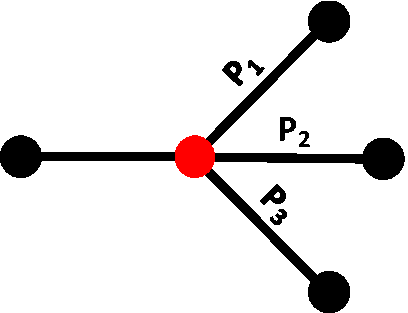
\includegraphics[scale=0.5]{decision3.pdf}
	\caption{Decision of an ant approaching a traffic node of degree 4 (represented in red) from the left hand side, with the probabilities $P_1$ to $P_3$ of the next edge.}
\end{figure}
Notice, that although the graph is not directed the decision of taking the same edge back to where the ant came from is not allowed. This edge is not part of the decision set.
Because we represent the terrain on which the ants move by a graph, the implementation of direction based turns is very difficult. Therefore we set $P_0 = 1$ in equation \ref{UTurn} and are left with the pheromone based U-turn equation.

Also we need the possibility of multiple colonies in the graph. Doing so the colonies and the food source are merged to one type of node. Every colony sees all nodes, except for their home node as food source. This has to be done, to simulate a not centralized network like the Swiss train system, where there are more then one train station.

Since the topic of this paper is the investigation of global and local reallocation in a graph we have to add that functionality to our model. Local redistribution happens, when an ant reaches a food source. With a probability depending on the difference in the productivity per ant of both colonies the ant will be reallocated to the new colony. In contrary to the local approach, the ants do not have to walk to their new home in the global solution. Instead the reallocation happens, when the ant arrives at its own nest. If the productivity of that ant is lower, then the global average productivity, The ant can be transferred to a new colony.
\subsection{Relation to the Swiss rail network}\label{relationNetwork}
The Swiss rail network should be described with the help of this model. The network is given as a graph, which connects all train station to each other. The following analogies between the ant and the train model have been made:
\begin{itemize}
  \item The train stations are represented by sources, as well as colonies.
  \item The trains are represented by ants.
  \item The travelling passengers are represented by food.
\end{itemize}
 In the new model the train stations are the starting point and the destination of all trains. Therefore there is no more distinction between colonies and sources, since colonies are sources for ants of a different colony. When a train reaches its destination, it gets filled up with people. With every arrival of trains at a station the amount of food at this station decreases, as there are less passengers waiting to be transported. This devaluation of the stations is counteracted by a regeneration rate, which is proportional to the popularity of the station. A popular station has a high regeneration rate, as there are lots of new potential passengers arriving in a given time step. With those analogies the productivity, which was defined as food carried to each colony per time is defined as people transported to each station per time. This is exactly the quantity, which we want to optimize.